\documentclass[../thesis.tex]{subfiles}

\begin{document}

  \chapter{Experimental results}
  \label{ch:experimental-results}


    \section{Experimental approach}
    \label{sec:conducted-measurements}

        For the first time during the team's research on alumina membranes, systematic measurements were conducted. Due to the limited period of time, only some aspects of the membranes could be investigated in more detail. During the internship, I measured 25 membranes of 3 wafers using the experimental setup described in \cref{sec:experimental-setup}. \Cref{tbl:wafer-specifications} summarizes the main fefatures of these wafers.

        \subfile{tikz/wafers/membrane_distribution.tex}

        \begin{table}[tb]
          \caption{Wafer specifications. The wafers thickness $l_\mathrm{pore}$, floating time $t_\mathrm{float}$ of the \textit{barrier layer} dissolution process and pore diameter dispersion $\Delta d_\mathrm{pore}^\mathrm{MEB}$ measured by electron beam microscopy are noted. The latter two parameters apply to the open pore membranes of the respective wafer.}
          \label{tbl:wafer-specifications}
          \selectfontsize{10pt}
          \begin{tabu} {X[r]X[r]X[r]X[r]}
            \unitoprule \\
            \textbf{Wafer} & \textbf{$l_\mathrm{pore}$ $[\si{\micro\meter}]$} & \textbf{$t_\mathrm{float}$ $[\si{\minute}]$} & \textbf{$\Delta d_\mathrm{pore}^\mathrm{MEB}$ $[\si{\nano\meter}]$} \\
            \unimidrule \\
            292 &60  &36+4   &- \\
            294 &60  &33   &-  \\
            295 &30  &35 (38 for b)  &7  \\
            296 &60  &40  &-  \\
            \unitoprule \\
          \end{tabu}
        \end{table}

        Victor Doebel's measurements had already shown strong dispersions in the properties of the membranes of different wafers, but also within the same wafer. Therefore, to evidence a possible systematic dispersion depending on the positions of the membranes on the wafers, the membranes are labelled according to the convention shown in \cref{fig:membrane-distribution}. Moreover, special attention was brought to the inhomogeneities on the wafers and the effect of the phosphoric acid etching used for the \textit{barrier layer} dissolution (ref???). A processing scheme for the wafers 295 and 296, which also marks the conducted measurements, is given by \cref{fig:wafer-processing-plans}.
        \medskip

        OR
        \medskip

        Victor Doebel's inital measurements previous to this internship had already shown strong dispersions in the properties of the membranes of different wafers, but also within the same wafer. Therefore, my goal was to perform systematic measurements on alumina membranes to determine the source of these dispersions. To probe a possible dependency on the position of the membranes on the wafers, the labeling is done according to the convention shwon in \cref{fig:membrane-distribution}.

        Due to the limited period of time, I chose to focus on the production steps of the \textit{barrier layer} dissolution and the pore diameter reduction by atomic layer deposition. During the intership, I measured 25 membranes of 4 wafers using the experimental setup described in \cref{sec:experimental-setup}. \Cref{tbl:wafer-specifications} summarizes the main characteristics of these wafers. A processing scheme for the wafers 295 and 296, which also marks the conducted measurements, is given by \cref{fig:wafer-processing-plans}.
        \medskip

        \subfile{tikz/wafers/wafer_processing_plans.tex}

        At first glance, resolving the bad open pore issue seems as easy as simply increasing the membranes' floating time during the \textit{barrier layer} dissolution. On second thought though, a problem comes up: \Cref{fig:294-sem} clearly states that some pores open before others. Therefore, these open pores are infiltrated by phosphoric acid which starts etching the pore from the inside increasing its diameter. This results in a broadening pore diameter distribution on the membrane caused by the \textit{barrier layer} dissolution process.

        \begin{figure}[tb]
          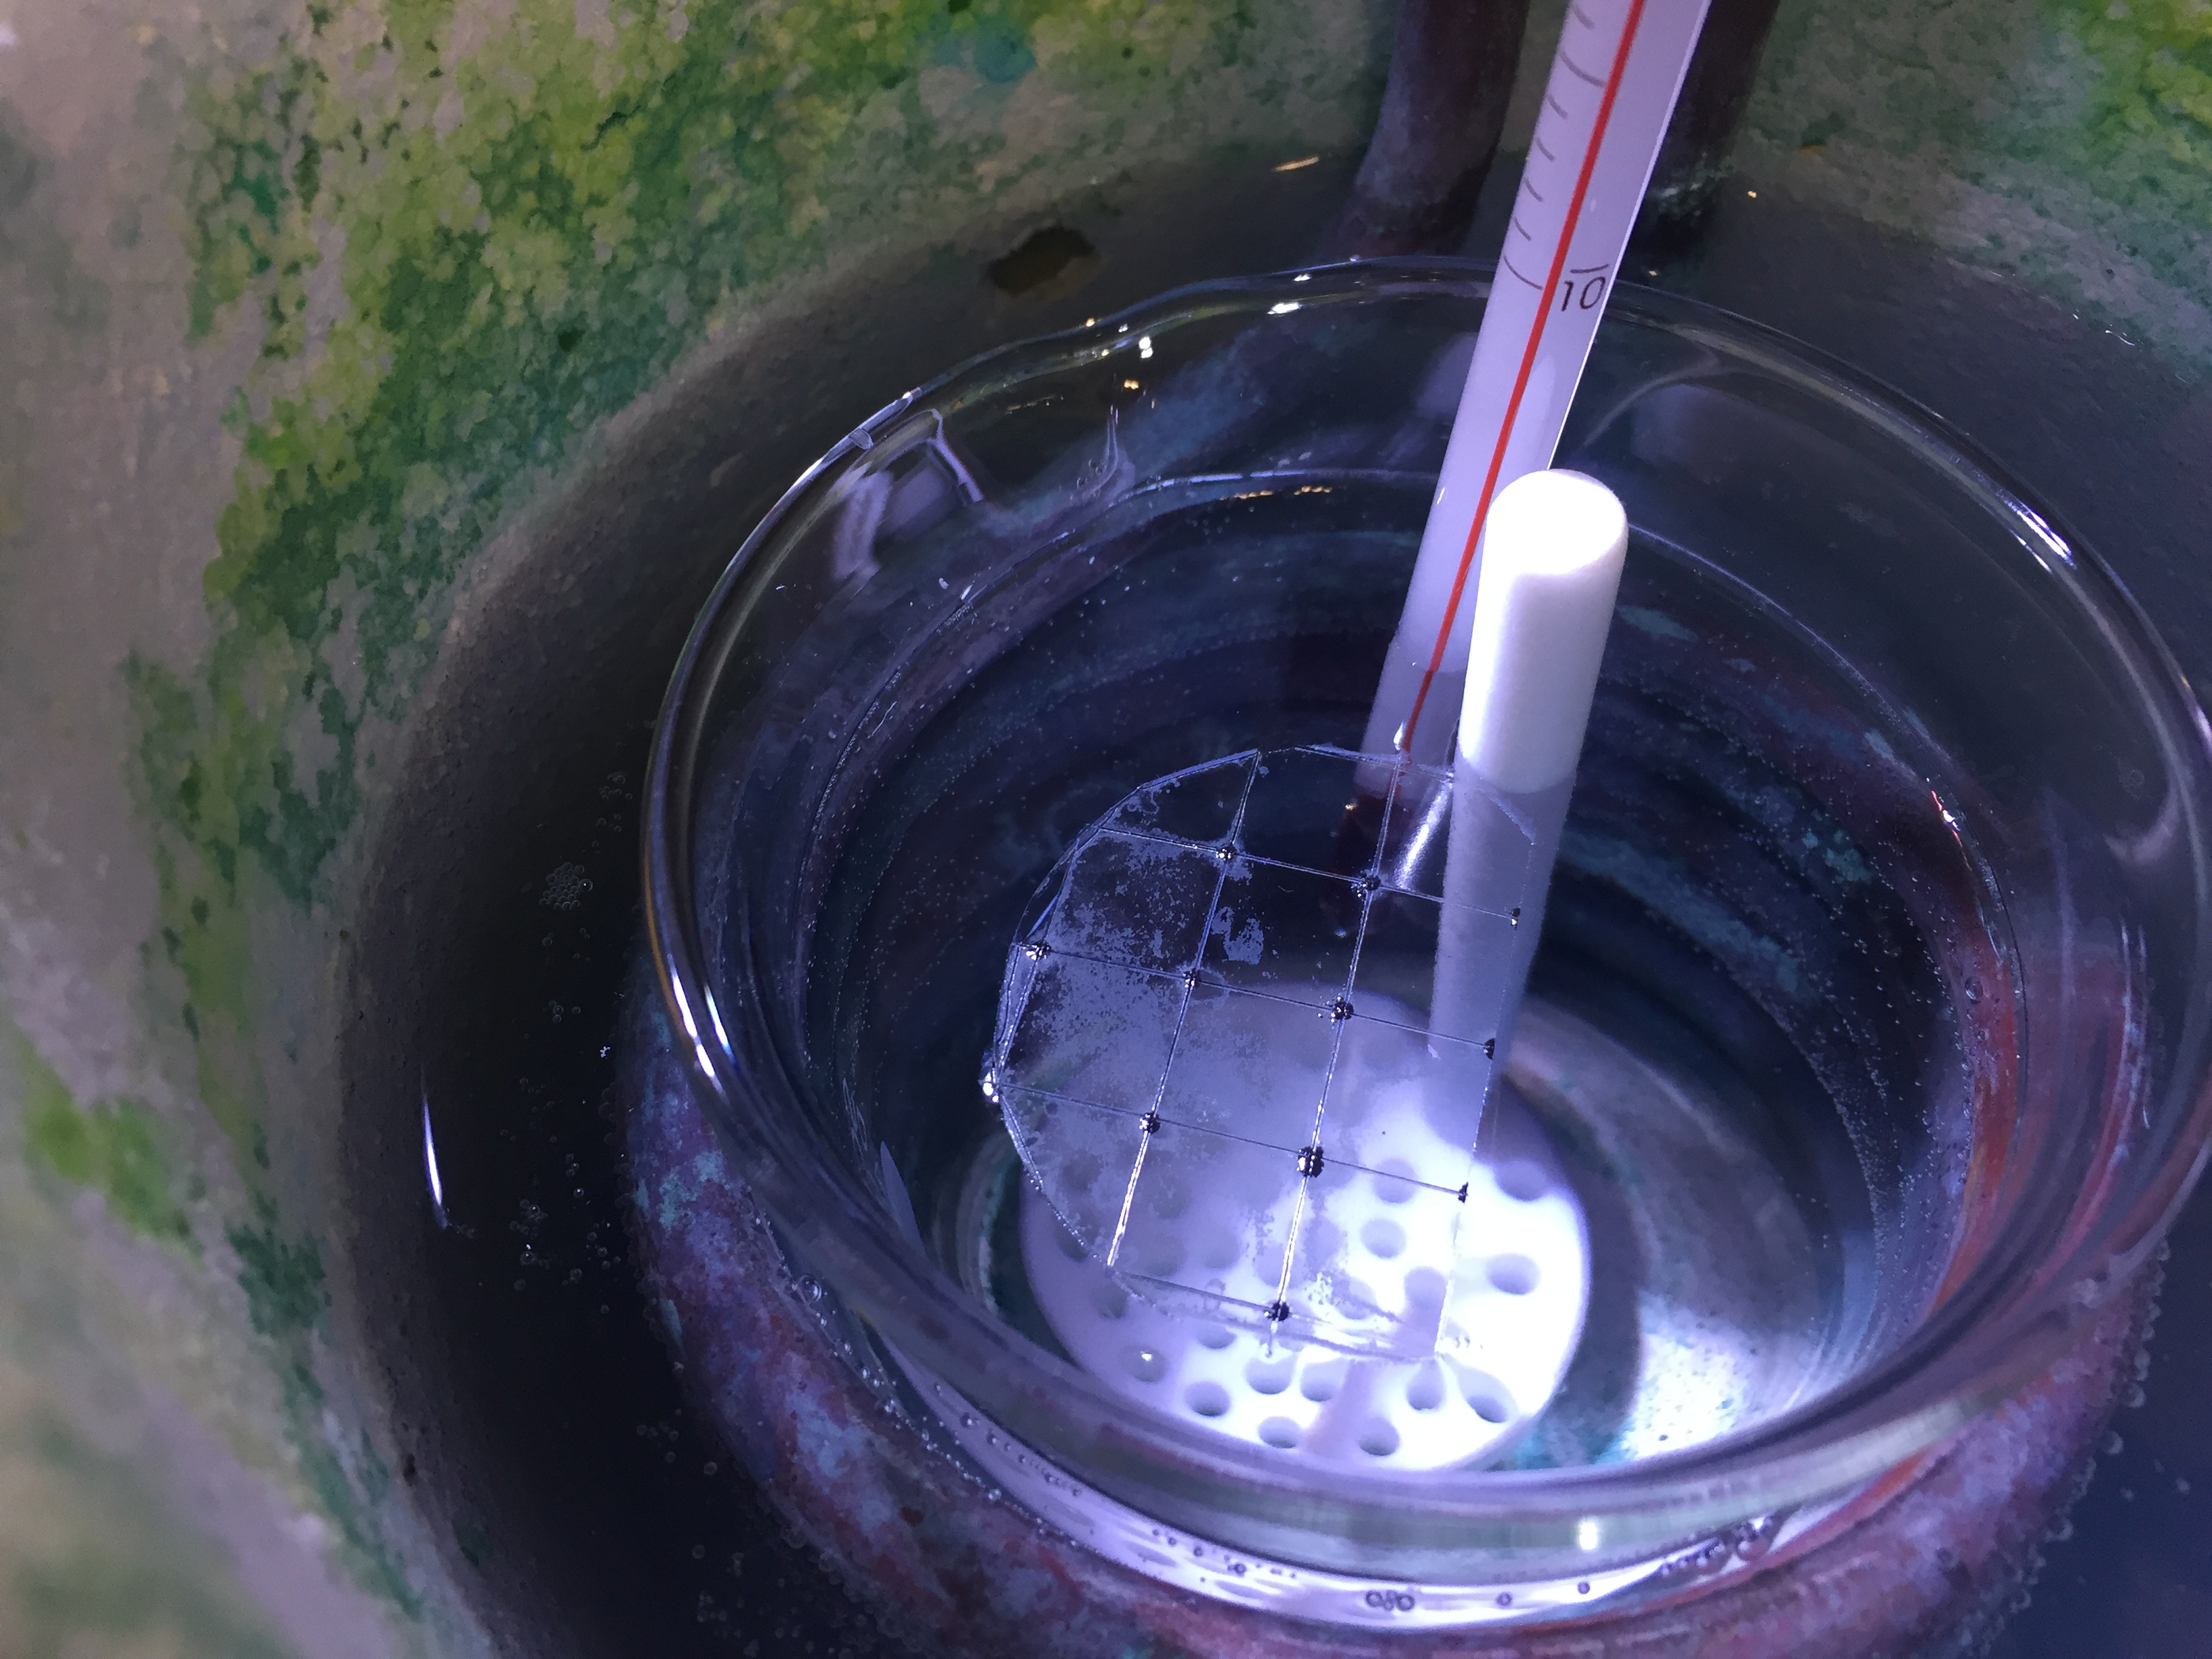
\includegraphics[width=0.9\textwidth]{images/milky_aspects.JPG}
          \caption{SEM image of a membran floated on phosphoric acid until the appearance of milky aspects.}
          \label{fig:milky-meb}
        \end{figure}

        As mentioned in ???MEMBRANE PRODUCTION, milky aspects occur at some point of the floating. Same as for spinodal condensation in the membranes, the filling of the opening pores with acid is assumed to cause light scattering and can therfore be linked to these milky aspects. Proof of this theory is the SEM image taken of a membrane that has been floated until the milky aspects appeared. Shown in \cref{fig:milky-meb}, the image confirms the semi open state of the membrane. As the milky aspects last for about
        \begin{equation*}
          t_\mathrm{milky} =\SI{3}{\minute}
        \end{equation*}
        and the etch rate of phosphoric acid on alumina is expected to be
        \begin{equation*}
          e=\SI{1}{\nano\meter\per\second},
        \end{equation*}
        the \text{barrier layer} dissolution process should cause an increase of the pore diameter dispersion of
        \begin{equation*}
          \Delta d_\mathrm{pore} = \SI{6}{nano\meter}.
        \end{equation*}
        This is quite dramatic regarding that the pore diameter distribution of a closed pore limited to about $\SI{10}{\nano\meter}$ ??? PROOVE!. Therefore, this increase should be obvious on the comparison of the evaporation branches of a closed pore membrane with an equivalent open pore membrane. Using \cref{fig:295b-closed-pores} as an example does not confirm these expectations which leads to the suspicion that the etch rates parallel to the pore axis $e_\parallel$ and perpendicular to the axis $e_\perp$ are different.


         To avoid this, one might think of immersing the membrane in order to fill every pore at the same time. While the pores would be widened during the whole \textit{barrier layer} dissolution process then, the distribution remained unchanged. However, the etch rate of phosphoric acid on alumina is expected to be approximately
        \begin{equation*}
          e=\SI{1}{\nano\meter\per\minute}
        \end{equation*}
        which makes for a pore diameter increase of infiltrated pores of
        \begin{equation*}
          \dot\Delta d_\mathrm{pore}=\SI{2}{\nano\meter\per\minute}.
        \end{equation*}
        From SEM images the thickness of the \textit{barrier layer} has been determined to be
        \begin{equation*}
          d_\mathrm{barrier-layer}=\SI{30}{\nano\meter},
        \end{equation*}
        so to open the pores at least $\SI{15}{\minute}$ translating to a pore diameter increase of
        \begin{equation*}
          \Delta d_\mathrm{pore} = \SI{30}{\nano\meter}.
        \end{equation*}
        As the aim is rather to produce membranes with pore diameters $d_\mathrm{pore}<\SI{10}{\nano\meter}$, the pure immersion becomes a backup plan.

        Instead, I delveloped the idea of a combination of floating to decrease the thickness of the barrier layer and immersion to do the final pore opening.



    \section{Membrane structure analysis}

      \subsection{Isotherm of an open pore membrane}
      \label{subsec:open-pore-isotherm}

        To start with, an isotherm of an open pore membane is compared to theory. According to \cref{eq:cond-evap-non-ideal-pore}, expectations are that condensation and evaporation occur at pressures smaller than the saturated vapor pressure $P_\mathrm{sv}$. Moreover, the condensation occuring at spiniodal pressure $P_\mathrm{sp}$ and the evaporation at $P_\mathrm{eq}$ implies a hysteresis. For the transmission measurement, two drops of transmission corresponding to condensation and evaporation are expected. Furthermore, the transmission should increase for the filled membrane in respect to its empty state.

        \Cref{fig:295b-open-pores} shows the measured isotherm of open pore membrane 296b'. As expected, condensation and evaporation occur at pressures
        \begin{equation*}
          P_\mathrm{rel,eq}^\mathrm{296b'} < P_\mathrm{rel,sp}^\mathrm{296b'} < P_\mathrm{rel,sv}
        \end{equation*}
        yielding a hysteresis. The dashed lines in \cref{fig:295b-open-pores} mark the average condensation and evaporation pressures of the isotherm. For their determination, the steepest point of the liquid fraction graph is sought, which corresponds to the minima of the transmission signals as expected. Converting these to diameters using \textsc{Kelvin} equation yields
        \begin{align*}
          d_\mathrm{pore}^\mathrm{296b'}(P_\mathrm{rel,sp}^\mathrm{296b'}=0,956)=\SI{44,4}{\nano\meter}, \\
          d_\mathrm{pore}^\mathrm{296b'}(P_\mathrm{rel,eq}^\mathrm{296b'}=0,925)=\SI{51,3}{\nano\meter},
        \end{align*}
        which makes for reasonable results. Furthermore, the transmission behaves according to theory in regard of the filled transmission in filled state being stronger than for the empty state.  (COMPARE TO SEM OF 296e???)
        \medskip

        \subfile{tikz/graphs/open_pore/296b_op.tex}

        \begin{figure}[p]
          \centering
          \subfloat[]{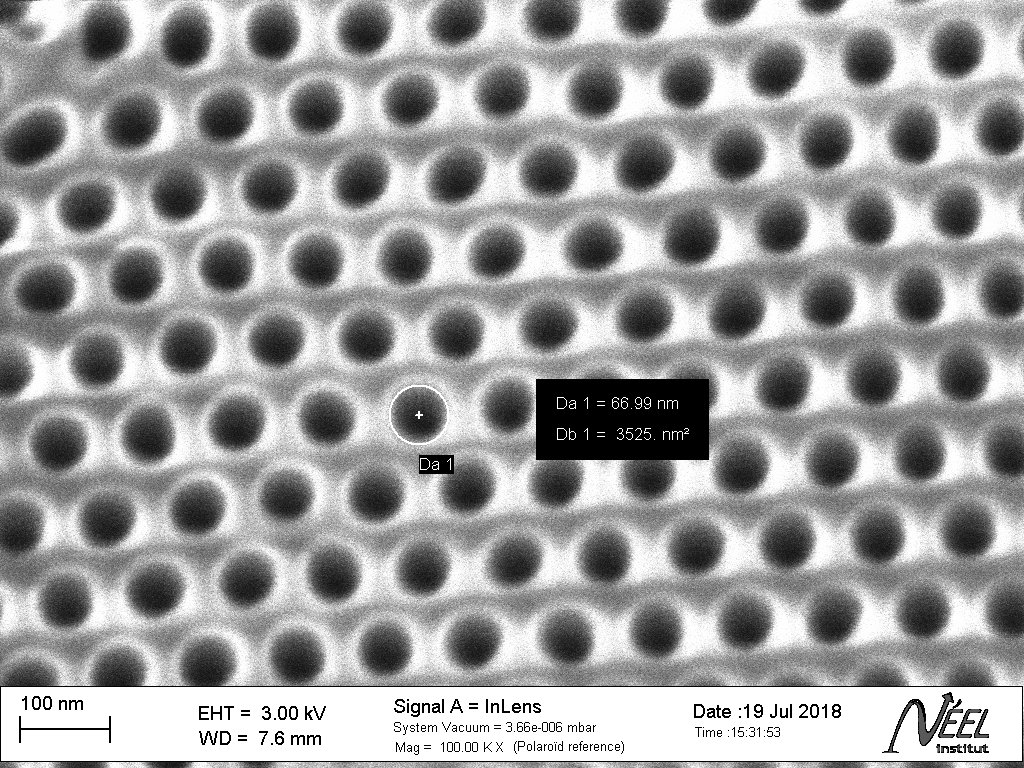
\includegraphics[width=.9\textwidth]{images/295g_pores_sol_side.jpg}
          \label{fig:295g-sol-side-sem}}
          \\
          \subfloat[]{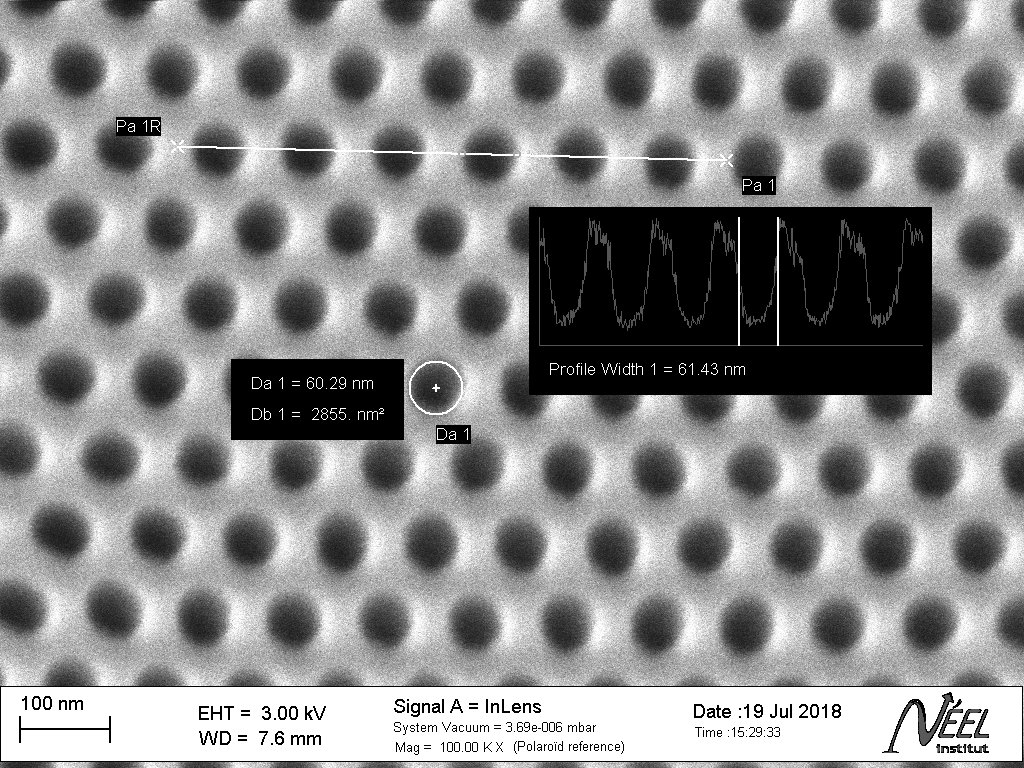
\includegraphics[width=.9\textwidth]{images/295g_pores_al_side.jpg}
          \label{fig:295g-al-side-sem}}
          \caption{SEM images of membrane 295g' implying the pores' funnellization. The pores on the solution side \protect\subref{fig:295g-sol-side-sem} show bigger diameters than those on the aluminum side \protect\subref{fig:295g-al-side-sem}.}
          \label{fig:295g-sem-funnellization-proof}
        \end{figure}

        By theory, the condensation and evaporation are expected to be vertical. The inclination of the two isotherm branches is explained as follows. Evaporating at equilibrium pressure leads to an inclined isotherm branch if there are either funnelled pores or the pores' diameters are distributed. On the other hand, condensation at spinodal pressure in weakly funnelled cylindrical pores (compare \cref{subsec:open-funnelled-pore-theory}) only shows an inclination if the pore sizes are distributed. At this point, the funnellization could be excluded to explain the observed isotherm. SEM images of various open pore membranes show a difference between the diameters of the solution and the aluminum side, which implies the presence of the pores' funnellization. \Cref{fig:295g-sem-funnellization-proof} shows the respective images of membrane 295g', supporting the assumption of pore funnellization.



    \subsection{Isotherm of a closed pore membrane}
    \label{subsec:closed-pore-isotherm}

        Moving on to a closed pore membrane, according to \cref{eq:cond-evap-non-ideal-pore}, no hysteresis is expected as both, condensation and evaporation occur at equilibrium pressure
        \begin{equation*}
          P_\mathrm{eq}<P_\mathrm{sv}
        \end{equation*}
        and should therefore be superimposed with the evaporation branch of an equivalent open pore membrane. For the transmission signal, the same behaviour as for the open pore membrane is expected: Two drops at condensation and evaporation respectively and a higher value in the filled state than in the empty state.

        \Cref{fig:295b-closed-pores} shows the isotherm of a closed pore membrane 296b along with an open pore membrane 296b'. First, condensation indeed shifts to lower pressures for the closed pore membrane. Moreover, the evaporation branch is also shifted to lower pressures. As will be explained in ???, this is due to the pore widening upon the \textit{barrier layer} dissolution process. As for the transmission, the drops' positions correspond to those of the volumetric isotherm's rises and filled state transmission is stronger than empty state transmission. However, the drastic increase in magnitude of the transmission signal upon the pore opening is not clear.
        \medskip

        That the hysteresis does not disappear is assumably due to intra pore corrugations. The latter vary the equilibrium pressure $P_\mathrm{eq}(d_\mathrm{pore})$ along the pore's length, which then causes the hysteretic behaviour. The phenomenon has been observed and explained this way by various experimentators REF???.

        \subfile{tikz/graphs/closed_pore_isotherm/cp_isotherm.tex}


    \subsection{Measurement reproducibility}
    \label{subsec:measurement-reproducibility}

        To check the reproducibility of the isotherm measurements, membranes were measured multiple times. \Cref{fig:292c-repro} shows four consecutive measurements for the same open pore membrane 292c and one more independent measurement ($LF_\mathrm{cond/evap}^\mathrm{292c,5}$). All the curves are close to superimposed. The biggest offset occurs before the condensation at spinodal pressure. As this part of the isotherm is not so important for the analysis, one can say that the volumetric measurements are very reproducable.

        \subfile{tikz/graphs/292c/292c_repro.tex}

        ADD OPTICAL MEASUREMENT??? not possible for 292c, would have to use other membranes with a maximum of two consecuctive measurements...


    \subsection{Inhomogeneities on one wafer}
    \label{subsec:wafer-inhomogeneities}

        \subfile{tikz/graphs/wafer_inhomogeneities/inhomogeneities_cp.tex}

        To start with, the wafers shall be tested for inhomogeneities. Therefore, isotherms of one wafer's membranes, which are in the same technical state, and have undergone exactly the same treatments, are compared. This is done for both: Closed pore membranes and open pore membranes. Because opening the membranes' pores involves one more production step, here, closed pore membranes are regarded first.

        \Cref{fig:inhomogeneities-cp} shows a comparison of closed pore membranes for wafer 295 and 296. Even though the membranes 296e' and 296f' had already been treated using phosphoric acid at the time of the measurements, the pores are still be closed as will be explained in \cref{sec:comparison-cp-op}.

        While for both wafers the overall shape of the different membranes' measurements matches, with one exception being membrane 295c, they are distributed along a short distance of the $P_\mathrm{rel}$-axis. As long as the shapes and also the size of the hysteresis of the volumetric isotherm match, this can be explained by differing pore size distributions. Membrane 295c is not analysed at this point, as it will be dealt with in detail in ???\cref{sec:theory-and-defects}. Unclear at this point is the extreme variation in magnitude of the transmission signal between the membranes (compare 296f' and 296b).
        \medskip

        In conclusion, to measure the effect of treatments on a given membrane, before and after measurements are necessary. It is not enough to measure one membrane representatively for multiple membranes in the same state.
        \subfile{tikz/graphs/wafer_inhomogeneities/inhomogeneities_op.tex}


    \subsection{Defects}
    \label{subsec:defects}

        All in all, the conducted measurements yield great results. The measured isotherms go along with the model introduced in \cref{eq:cond-evap-non-ideal-pore} and are reproducible. The inhomogeneity on a given wafer is bearable???.

        Nevertheless, pore defects and dispersions were detected. First, there is the pore size distribution. To estimate its broadness, SEM images are analyzed in 295g???. Next, the funnellization and the corrugation must be mentioned. Both cause intra pore diameter variations that cause inclined isotherms, even for a single pore. Last, bad open pores were detected during the measurements. This problem will be discussed in the following section, as its examination leads to valuable, relevant results.


  \section{The problem of pore opening}
  \label{sec:opening-problem}


      \subsection{Bad open pores}
      \label{subsec:bad-open-pores}

        \subfile{tikz/graphs/294_bad_open_pores/294_bad_open_pores.tex}

        Victor Doebel's measurements before my internship revealed membranes with bad open pores. The term \textit{bad open pores} refers to a membrane that has been floated on phosphoric acid for the \textit{barrier layer} dissolution not long enough to completely open the pores. ???TIKZ IMAGE??? As a result some pores remain closed whereas others have constricted openings and some are fully open. \Cref{fig:294-bad-open-pores} shows the comparison of closed pore membrane 294cp and membrane 294op with bad open pores. The assumption is derived from the isotherm in the following way: By theory, the condensation branch should be shifted towards higher pressure for open pores in respect to closed pores. While this is the case for membrane 294op's end of the condensation rise, it still starts at the same pressure as the condensation of the closed pore membrane which by theory condenses at equilibrium pressure. Moreover, the evaporation of 294op is superimposed with the one of 294cp. While this is expected by theory, it rules out the possibility of an increase in funnellization or corrugation causing the broader condensation branch of the open pore membrane. The only possible explanation for the observed behaviour is a population of open pores alongside one of closed pores on the membrane. In this case some pores start filling at equilibrium pressure, wheras others fill at higher spinodal pressures depending on the size of the pore opening on the aluminum side. independently, SEM images of the membrane confirm the assumption of bad open pores as shown in \cref{fig:294-sem}.

        \begin{figure}[tbp]
          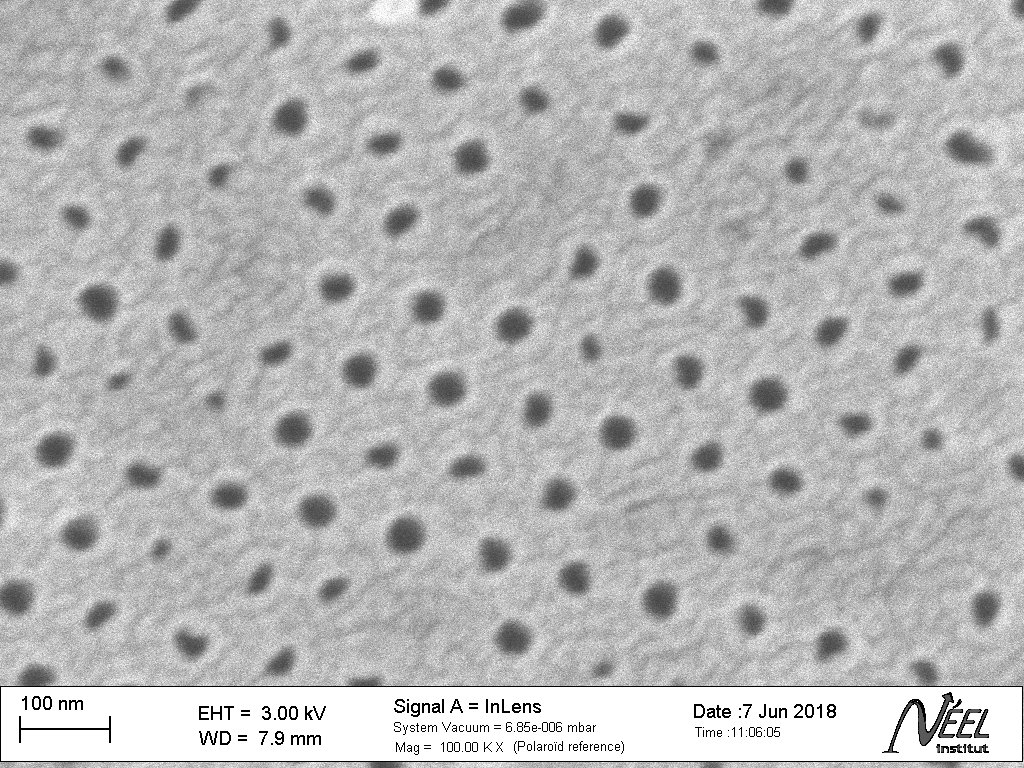
\includegraphics[width=0.9\textwidth]{images/294_bad_open_pores.jpg}
          \caption{SEM image confirming the bad open pores of membrane 294op.}
          \label{fig:294-sem}
        \end{figure}

\end{document}
